% Chapter 1

\chapter{SCPI (Standard Commands for Programmable Instruments)
} % Write in your own chapter title
\label{Capitolul2}
\lhead{Capitolul 2. \emph{SCPI (Standard Commands for Programmable Instruments)}} % Write in your own chapter title to set the page header

Domeniul instrumenta\c{t}iei a folosit dintotdeauna tehnologie electronic\u{a} larg utilizat\u{a}. Principiul acului de ceas a fost folosit la scar\u{a} larg\u{a} pentru construirea de instrumente de m\u{a}surat analogice. Capacitorul variabil, rezistorul variabil au fost utilizate primele \^{i}n dezvoltarea instrumenta\c{t}iei electronice. Apoi tehnologia display-ului a fost \^{i}mprumutat\u{a} din televiziune \^{i}n vederea utiliz\u{a}rii pentru aparatele de analizat \c{s}i cele osciloscop.

Astazi, sistemele viabile de calcul desktop \c{s}i notebook constituie, printre altele suportul pentru noua genera\c{t}ie de instrumente - instrumentele virtuale. Acestea sunt proiectate \c{s}i realizate de utilizator conform cu nevoile specifice.

\^{I}n 1965, Hewlett-Packard dezvolta HPIB (Hewlett Packard Interface Bus) \^{i}n vederea conectarii instrumentelor programabile la sistemele de calcul. Datorit\u{a} ratei mari de transfer, nominal 1 Mbytes/s, aceast\u{a} interfa\c{t}\u{a} a c\^{a}\c{s}tigat imediat popularitate. Ulterior s-a impus ca standardul numit IEEE 488, apoi evolu\^{a}nd la IEEE 488.1. Ast\u{a}zi se utilizeaz\u{a} mai larg denumirea de GPIB (General Purpose Interface Bus) \^{i}n locul celei de HPIB. 

Standard Commands for Programable Instruments a luat structura de comenzi definit\u{a} \^{i}n cadrul IEEE 488.2 \c{s}i a creat un mediu de programare unic, transparent. SCPI, fiind independent de partea hardware, poate fi implementat peste alte tipuri de standarde, cum ar fi RS-232 sau GPIB. Mai concret, SCPI \emph{define\c{s}te un set standard de comenzi pentru controlul dispozitivelor de testare \c{s}i m\u{a}surare \^{i}n sistemele de instrumente}.

Un sistem de instrumente reprezint\u{a} un grup de dispozitive de testare \c{s}i m\u{a}surare, conectate printr-o magistral\u{a} de comunica\c{t}ie la un calculator de control, apelat de controlerul de sistem. Un sistem de instrumente poate include dispozitive de sine-st\u{a}t\u{a}toare, cum ar fi instrumente de tip IEEE 488, sau placi-instrumente, \^{i}nglobate \^{i}ntr-un sistem.

Controlerul de sistem trimite comenzi unuia sau mai multor instrumente prin intermediul magistralei. Aceste comenzi sunt numite mesaje de program. Instrumentele trimit \^{i}napoi r\u{a}spunsuri c\u{a}tre magistral\u{a}. Mesajul r\u{a}spuns poate fi rezultatul unei m\u{a}sur\u{a}tori, o setare a instrumentului sau un mesaj de eroare. C\^{a}nd un mesaj de program genereaza direct un raspuns, acesta se nume\c{s}te interogare. SCPI reprezint\u{a} un limbaj uniform \c{s}i consistent pentru controlul instrumentelor de testare \c{s}i m\u{a}surare.

\section{Scopul SCPI}
Principalul scop al SCPI este s\u{a} reduc\u{a} generarea sistematica a programelor pentru echipamente automate de testare (Automatic Test Equipment - ATE). Instrumentele SCPI sunt foarte flexibile, accept\^{a}nd un domeniu larg de formate de comenzi \c{s}i parametri.

Cheia unei astfel de program\u{a}ri consistente const\u{a} \^{i}n reducerea diferitelor modalit\u{a}\c{t}i de a controla func\c{t}iile instrumentelor. Filosofia SCPI este ca acelea\c{s}i func\c{t}ii ale unui instrument s\u{a} fie controlate de acelea\c{s}i comenzi SCPI.

SCPI este proiectat \^{i}n vederea adaug\u{a}rii de noi comenzi \^{i}n orice perioad\u{a} de timp, f\u{a}r\u{a} ca acestea s\u{a} cauzeze probleme de programare a instrumentelor. Pe m\u{a}sura ce apar noi instrumente, exist\u{a} inten\c{t}ia de a men\c{t}ine compatibilitatea programului de control cu alte instrumente SCPI deja existente.

Avantajul folosirii SCPI pentru programatorul sistemului ATE este reducerea timpului de \^{i}nv\u{a}\c{t}are de a programa noi instrumente SCPI, chiar dup\u{a} programarea unui alt instrument tot de tip SCPI.

Furniz\^{a}nd un mediu consistent de programare, \^{i}nlocuirea unui instrument SCPI cu alt echipament SCPI \^{i}ntr-un sistem ATE va necesita de obicei mai pu\c{t}in efort dec\^{a}t cu instrumente non-SCPI.

Toate instrumentele SCPI trebuie s\u{a} fie \^{i}n conformitate cu specifica\c{t}iile IEEE 488.2 \c{s}i vor pune \^{i}n aplicare toate comenzile comune declarate obligatorii:

\begin{table}[h]
	\begin{center}
	\begin{tabular}{|l|l|}
		\hline
		Mnemonica & Nume\\
		\hline
		*CLS & Clear Status Command\\
		*ESE & Standard Event Status Enable Command\\
		*ESE? & Standard Event Status Enable Query\\
		*ESR? & Standard Event Status Register Query\\
		*IDN? & Identification Query\\
		*OPC & Operation Complete Command\\
		*OPC? & Operation Complete Query\\
		*RST & Reset Command\\
		*SRE & Service Request Enable Command\\
		*SRE? & Service Request Enable Query\\
		*STB? & Read Status Byte Query\\
		*TST? & Self Test Query\\
		*WAI & Wait-to-Continue Command\\
		\hline
	\end{tabular}
	\end{center}
	\caption{Lista de comenzi obligatorii}
\end{table}

\begin{figure}[!htb]
	\centering
	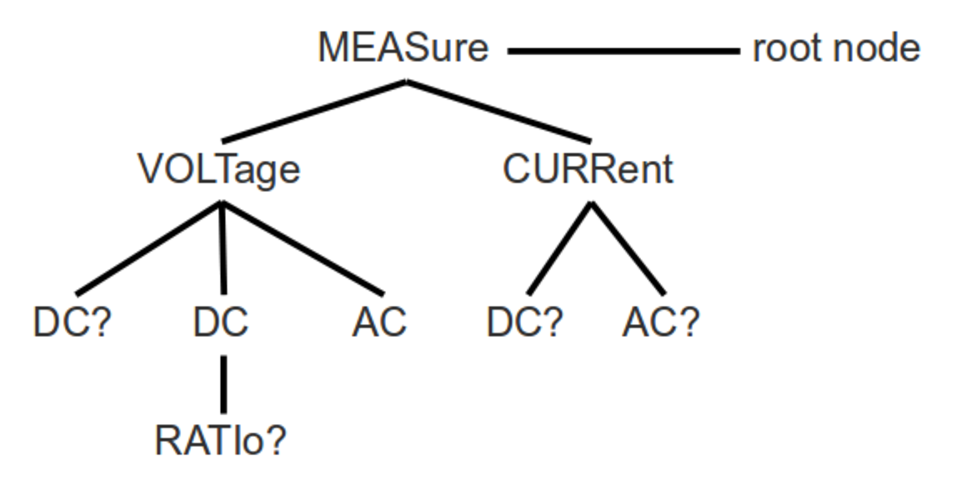
\includegraphics[scale=0.8]{./Figuri/structuracomanda.eps}
	\caption{Structura unei comenzi SCPI}
	\label{structuracomanda}
\end{figure}

\section{Comenzi suprapuse \c{s}i secven\c{t}iale}
IEEE 488.2 define\c{s}te o deosebire \^{i}ntre comenzile suprapuse \c{s}i cele secven\c{t}iale. A\c{s}a cum este definit\u{a} \^{i}n standard, o comand\u{a} secven\c{t}ial\u{a} este una care \^{i}\c{s}i termin\u{a} executarea \^{i}nainte de pornirea comenzii urm\u{a}toare. O comand\u{a} suprapus\u{a} este una care nu termin\u{a} executarea \^{i}nainte de \^{i}nceperea comenzii urm\u{a}toare.

IEEE 488.2 define\c{s}te trei comenzi comune, *OPC, *WAI, *OPC?, pe care un dispozitiv conduc\u{a}tor \^{i}l poate folosi pentru a-\c{s}i sincroniza func\c{t}ionarea la executarea de comenzi suprapuse.

Fiecare comand\u{a} suprapus\u{a} a fost asociat\u{a} cu un Pending Operation Flag. Dispozitivul configureaz\u{a} acest steag la valoarea \emph{true} atunci c\^{a}nd trece de la comanda corespunz\u{a}toare din blocul Execution Control c\u{a}tre blocul Device Action. Dispozitivul configureaz\u{a} steagul pe valoarea \emph{false} c\^{a}nd func\c{t}ionarea dispozitivului este terminat\u{a} sau este intrerupt\u{a}.

\section{Comenzi optionale}
Exist\u{a} comenzi facultative, depinz\^{a}nd de posibilita\c{t}ile instrumentului. C\^{a}nd un dispozitiv nu suport\u{a} to\c{t}i parametrii alternativi care sunt permi\c{s}i pentru o comand\u{a} SCPI, el poate s\u{a} pun\u{a} \^{i}n aplicare o subselec\c{t}ie a acestor valori, numai cu excep\c{t}ia \^{i}n care au fost altfel declarate. De exemplu, dac\u{a} un instrument pune \^{i}n aplicare numai func\c{t}iile RECTangular \c{s}i UNIform pentru comenzile CALCulate:TRANSform:WINDow, se poate genera o eroare de la oricara alt parametru declarat (Flattop, Hamming, etc). Oricum, un dispozitiv trebuie s\u{a} pun\u{a} \^{i}n aplicare to\c{t}i parametrii unei comenzi SCPI multi-parametru.

Un instrument cu un monitor care este configurat s\u{a} fie \^{i}n permanen\c{t}\u{a} pornit nu are nevoie de punerea \^{i}n aplicare a unei comenzi pentru pornire/oprire. Dac\u{a} un instrument are o configura\c{t}ie fix\u{a}, \^{i}n care o setare nu corespunde cu valoarea *RST, atunci instrumentul va pune \^{i}n aplicare comanda pentru acea setare.

\subsection{Interpretarea tabelei de comenzi}
Tabelele de comenzi sunt folosite ca s\u{a} defineasc\u{a} un set de comenzi SCPI. Un tabel prezint\u{a} comenzile, rela\c{t}iile lor ierarhice, parametrii \^{i}nrudi\c{t}i (\^{i}n cazul \^{i}n care exist\u{a}), \c{s}i nota\c{t}ii sau comentarii asociate acestora. Tabelul este format din trei coloane: una pentru cuv\^{a}ntul cheie (Keyword), una pentru forma parametrului (Parameter Form) \c{s}i una pentru nota\c{t}ii sau comentarii (Notes).

Coloana cuv\^{a}ntului cheie (Keyword) furnizeaz\u{a} numele comenzii. Numele comenzii reale const\u{a} din unul sau mai multe cuvinte cheie, comenzile SCPI baz\^{a}ndu-se pe o structur\u{a} ierarhic\u{a}, cunoscut\u{a} de asemenea ca structur\u{a} arborescent\u{a}. \^{I}ntr-n astfel de sistem, comenzile asociate sunt grupate \^{i}mpreun\u{a} sub un nod comun \^{i}n ierarhie. Acestea \c{s}i ramurile asem\u{a}n\u{a}toare sunt conectate \^{i}ntr-un num\u{a}r mai mare sau mai mic, p\^{a}n\u{a} ce \^{i}nt\^{a}lnesc r\u{a}d\u{a}cina structurii arborescente. Cu c\^{a}t un nod este mai aproape de r\u{a}d\u{a}cin\u{a}, cu at\^{a}t este considerat mai important \^{i}n ierarhie. Pentru a ob\c{t}ine o ramur\u{a} special\u{a} sau o comand\u{a} special\u{a}, trebuie s\u{a} fie specificat\u{a} calea unde se afl\u{a}. Aceast\u{a} cale este reprezentat\u{a} \^{i}n tabele prin plasarea celui mai superior nod \^{i}n ierarhie, \^{i}n pozi\c{t}ia cea mai din st\^{a}nga. Nodurile inferioare \^{i}n ierarhie sunt mutate cu o pozi\c{t}ie \^{i}nspre partea dreapt\u{a}, dedesuptul nodului-parinte.

Parantezele drepte sunt utilizate pentru cuvintele cheie op\c{t}ionale atunci c\^{a}nd se programeaza comanda; instrumentul va trebui s\u{a} proceseze aceast\u{a} comand\u{a} ca av\^{a}nd acela\c{s}i efect, indiferent dac\u{a} nodul-op\c{t}iune este omis de programator. Un astfel de nod este denumit nod implicit (default node).

Majusculele din cadrul cuv\^{a}ntului cheie al unei comenzi indic\u{a} forma prescurtat\u{a} care este la fel de valabila ca \c{s}i forma complet\u{a}.

Coloana cu forma parametrului indic\u{a} numarul \c{s}i ordinea parametrului \^{i}ntr-o comand\u{a}, precum \c{s}i valorile sale. O comand\u{a} poate permite folosirea unui tip de parametru SCPI, literal, sau o combina\c{t}ie a celor dou\u{a}.
 
\^{I}n coloana cu forma parametrului, o serie de caractere au o semnifica\c{t}ie special\u{a}. Ca \c{s}i mai sus, parantezele drepte sunt folosite pentru a indica unul sau mai mul\c{t}i parametri care sunt op\c{t}ionali atunci c\^{a}nd se controleaz\u{a} instrumentul. Acoladele sunt folosite pentru indicarea parametrilor care sunt folosi\c{t}i de mai multe ori sau deloc. Bara vertical\c{a} poate fi interpretat\u{a} ca "sau" \c{s}i este folosit\u{a} pentru a separa diferite op\c{t}iuni ale parametrilor alternativi. 

Coloana nota\c{t}ii: forma interog\u{a}rii unei comanzi este generat\u{a} adaug\^{a}nd un semn de \^{i}ntrebare la ultimul cuv\^{a}nt cheie. Oricum, nu toate comenzile au o forma specific\u{a} a interog\u{a}rii, \c{s}i alte comenzi exist\u{a} numai sub forma de interogare.

Exemplu:
\begin{table}[h]
	\begin{center}
	\begin{tabular}{|l|l|l|}
		\hline
		KEYWORD & PARAMETER FORM & NOTES\\
		\hline
		:FREQuency &  & \\
		\verb [:CW] & \textless numeric value\textgreater & \\
		\ \ \ \ :AUTO & \textless Boolean\textgreater & \\
		:CENTer & \textless numeric value\textgreater & \\
		:SPAN & \textless numeric value\textgreater & \\
		\hline		
	\end{tabular}
	\end{center}
\end{table}

Pentru setarea valoarii frecven\c{t}ei pentru un semnal sinusoidal continuu (contnuous wave - CW), comanda ar trebui s\u{a} aiba urm\u{a}toarea forma: 
\begin{center}
FREQuency:CW 2000000
\end{center}
Deoarece nodul [:CW] este op\c{t}ional, se poate utiliza urm\u{a}toarea form\u{a} de comand\u{a}: 
\begin{center}
FREQuency: 2000000
\end{center}
Pentru setarea valorii AUTO, poate fi utilizat\u{a} una din urm\u{a}toarele forme, depinz\^{a}nd, ca \c{s}i mai sus, de nodul CW care este op\c{t}ional:
\begin{center}
FREQuency:CW:AUTO OFF

FREQuency:AUTO OFF
\end{center}
Forma interog\u{a}rii a comenzii AUTO este una din cele de mai jos: 
\begin{center}
FREQuency:CW:AUTO?

FREQuency:AUTO?
\end{center}

\section{Construirea structurii arborescente}
Comenzile SCPI sunt bazate pe o structur\u{a} ierarhic\u{a}. Aceasta permite ca acela\c{s}i cuv\^{a}nt cheie s\u{a} fie \^{i}ntrebuin\c{t}at \^{i}n repetate r\^{a}nduri pentru scopuri diferite, f\u{a}c\^{a}nd ca mnemonicele s\u{a} aibe o pozi\c{t}ie unic\u{a} \^{i}n ierarhie. Aceasta se realizeaz\u{a} \^{i}n vederea evit\u{a}rii suprapunerii cu oricare alta abreviere aflat\u{a} la acela\c{s}i nivel. Folosind comenzile ierarhice ar trebui s\u{a} se elimine nevoia de mnemonice cu mai multe cuvinte.

\section{Sintaxa mesajelor program}
Un mesaj program const\u{a} din una sau mai multe comenzi SCPI trimise de la controler la instrument pentru a comanda o ac\c{t}iune sau pentru a interoga instrumentul. \^{I}n figura \ref{fig1} este reprezentat schematic un mesaj program.

\begin{figure}[htp]
 \centering
 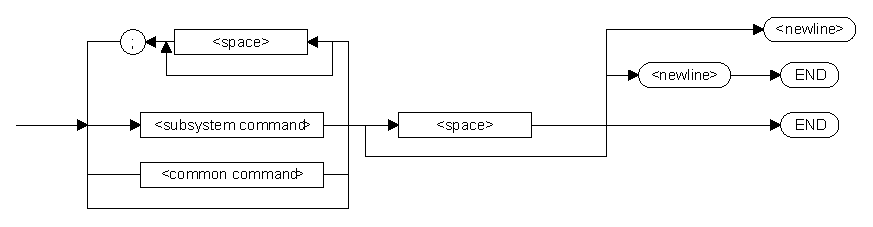
\includegraphics[scale=0.7]{Figuri/fig1_scpi_meas.eps}
 \caption{Sintaxa mesajului program}
 \label{fig1}
\end{figure}

Simbolul punct \c{s}i virgul\u{a} este folosit pentru separarea comenzilor din acela\c{s}i grup. De exemplu se poate trimite urm\u{a}torul mesaj pentru a seta starea portului de ie\c{s}ire digital (8 linii de ie\c{s}ire) \c{s}i pentru a citi starea portului:

\begin{center}
\begin{verbatim}
:OUTPut:255; :OUTPut?
\end{verbatim}
\end{center}

Unirea unor comenzi din grupuri diferite se realizeaz\u{a} folosind punct \c{s}i virgul\u{a} \c{s}i dou\u{a} puncte. De exemplu citirea registrului Operation Status \c{s}i setarea portului digital de ie\c{s}ire:

\begin{center}
\begin{verbatim}
:STATus:OPERation:CONDition? ;:OUTPut:255
\end{verbatim}
\end{center}

Pentru terminarea unui mesaj program se pot folosi urm\u{a}toarele terminatoare:
\begin{itemize}
	\item \textless  newline\textgreater sau caracterul \textless  NL\textgreater
	\item \textless  END\textgreater care este interpretat ca \c{s}i \textless  NL\textgreater
	\item \textless  newline\textgreater\textless  END \textgreater
\end{itemize}

Terminarea mesajului program reseteaz\u{a} calea comenzii SCPI curente la nivel radacin\u{a}.

Urm\u{a}toarele sec\c{t}iuni descriu sintaxa comenzilor SCPI generale \c{s}i comenzilor SCPI subsistem.

\subsection{Sintaxa comenzilor SCPI generale}
Figura \ref{fig2} descrie sintaxa comenzilor SCPI generale.

\begin{figure}[htp]
 \centering
 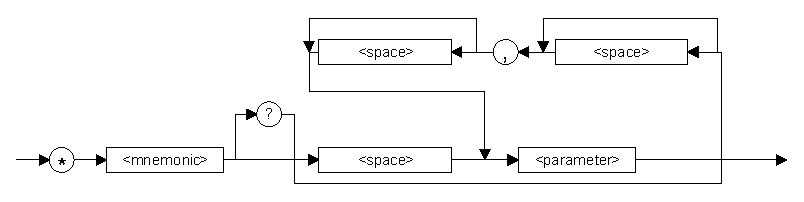
\includegraphics[scale=0.8]{Figuri/fig2_scpi_meas.eps}
 \caption{Sintaxa comenzilor generale}
 \label{fig2}
\end{figure}

Comenzile SCPI generale \^{i}ncep cu simbolul asterix (*). Comenzile sunt de tip case-insensitive. De exemplu urm\u{a}toarele comenzi produc acela\c{s}i rezultat:
\begin{verbatim}
*RST
*rst
*Rst
\end{verbatim}

Interog\u{a}rile necesit\u{a} simbolul \emph{semn de \^{i}ntrebare} la sf\^{a}r\c{s}itul comenzii:
\begin{verbatim}
*IDN?
\end{verbatim}

\subsection{Sintaxa comenzilor SCPI subsistem}
Figura \ref{fig3} descrie sintaxa comenzilor SCPI subsistem.

\begin{figure}[htp]
 \centering
 \includegraphics[scale=0.8]{Figuri/fig3_scpi_meas.eps}
 \caption{Sintaxa comenzilor SCPI subsistem}
 \label{fig3}
\end{figure}

Se folose\c{s}te simbolul \emph{dou\u{a} puncte} pentru separarea cuvintelor cheie:
\begin{verbatim}
:STATus:OPERation:ENABle
\end{verbatim}

Interog\u{a}rile necesit\u{a} simbolul semn de \^{i}ntrebare la sf\^{a}r\c{s}itul comenzii:
\begin{verbatim}
:STATus:OPERation:CONDition?
\end{verbatim}

\section{Sintaxa mesajelor r\u{a}spuns}
Un mesaj r\u{a}spuns const\u{a} din date \^{i}ntr-un format specific SCPI care au fost cerute instrumentului de c\u{a}tre controler.

Figura \ref{fig4} descrie sintaxa mesajului r\u{a}spuns al unui instrument:

\begin{figure}[htp]
 \centering
 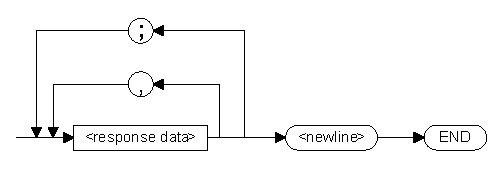
\includegraphics[scale=1]{Figuri/fig4_scpi_meas.eps}
 \caption{Sintaxa mesajului r\u{a}spuns}
 \label{fig4}
\end{figure}

Mesajele r\u{a}spuns pot con\c{t}ine at\^{a}t virgula c\^{a}t \c{s}i punct \c{s}i virgula ca \c{s}i separatori. C\^{a}nd o singur\u{a} comand\u{a} de interogare returneaz\u{a} valori multiple, se folose\c{s}te virgula pentru a separa fiecare element. C\^{a}nd sunt trimise mai multe interog\u{a}ri \^{i}ntr-un singur mesaj, grupurile de date corespunz\u{a}toare fiec\u{a}rei interog\u{a}ri sunt separate prin punct \c{s}i virgul\u{a}.

Terminatorul mesajului r\u{a}spuns este \^{i}ntotdeauna \textless  newline\textgreater\textless \^END\textgreater.

\section{Antete de program}
Antetele de program sunt cuvintele cheii care identific\u{a} comanda. Instrumentele vor accepta \c{s}i varianta cu comenzi cu majuscule \c{s}i cea cu litere mici, instrumentele nef\u{a}c\^{a}nd distinc\c{t}ie \^{i}ntre acestea.

Antetele de program se compun din dou\u{a} tipuri distincte \c{s}i anume antetele de comand\u{a} \c{s}i antetele de control ale instrumentului.

\begin{figure}[htp]
 \centering
 \includegraphics[scale=1]{Figuri/scpi_ro_1.eps}
 \caption{Sintaxa antetelor de comanda}
 \label{fig6}
\end{figure}

\begin{figure}[htp]
 \centering
 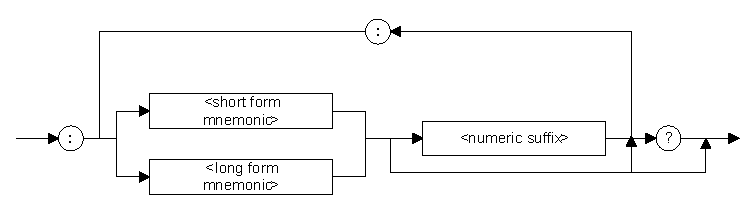
\includegraphics[scale=1]{Figuri/scpi_ro_2.eps}
 \caption{Sintaxa antetelor de control}
 \label{fig6}
\end{figure}

\section{Interog\u{a}rile}
Toate comenzile, numai \^{i}n cazul c\^{a}nd sunt altfel notate, au \^{i}n plus \c{s}i o form\u{a} de interogare. A\c{s}a cum este definit \^{i}n IEEE 488. 2, o interogare este un antet de comand\u{a} cu un simbol al unui semn de \^{i}ntrebare ad\u{a}ugat (de exemplu FREQ: CENT?). C\^{a}nd un formular de \^{i}ntrebare al unei comenzi este primit, setarea curent\u{a} asociat\u{a} comenzii este plasat\u{a} \^{i}n buffer-ul de ie\c{s}ire. R\u{a}spunsurile interog\u{a}rii nu includ antetul de comand\u{a}. Executare unui formular de \^{i}ntrebare nu are efectele secundare. O excep\c{t}ie este \^{i}n subsistemul MEASurement, unde set\u{a}rile instrumentului ar putea s\u{a} schimbe rezultatul m\u{a}sur\u{a}torii.

Atat formularul de comand\u{a} c\^{a}t \c{s}i cel de interogare trebuie s\u{a} fie implementate, excep\c{t}ie f\u{a}c\^{a}ndu-se \^{i}n cazul \^{i}n care un comentariu care indic\u{a} altceva apare \^{i}n sumarul cuvintelor ceie. Chiar \c{s}i c\^{a}nd o comand\u{a} accept\u{a} numai o singur\u{a} selec\c{t}ie, at\^{a}t formularul de comand\u{a} c\^{a}t \c{s}i cel de interogare vor trebui s\u{a} fie aplicate.

C\^{a}nd informa\c{t}iile de caracter se \^{i}ntrebuin\c{t}eaz\u{a} pentru un parametru, ambele variante, longform \c{s}i shortform, vor trebui s\u{a} fie recunoscute. Dac\u{a} comanda are un formular de \^{i}ntrebare cu informa\c{t}ii de r\u{a}spuns de caracter, valoarea shortform este \^{i}ntotdeauna \^{i}ntoars\u{a}.

C\^{a}nd parametrii numerici sunt interoga\c{t}i, rezultatul se va \^{i}ntoarce \^{i}n unit\u{a}\c{t}ile de m\u{a}sur\u{a} de baz\u{a}, \^{i}n cazul \^{i}n care nu se specific\u{a} sau impune altfel. C\^{a}nd unele din diferitele unit\u{a}\c{t}i pot fi considerate fundamentale (de exemplu: dBuV, dBm), atunci unit\u{a}\c{t}ile rezultatului vor trebui s\u{a} fie detaliate \^{i}n descrierea r\u{a}spunsului interog\u{a}rii.

\section{Parametrii}
 SCPI folose\c{s}te formele de parametri descrise \^{i}n standardul IEEE 488.2, cu cateva restric\c{t}ii adi\c{t}ionale. Trebuie observat c\u{a} SCPI specific\u{a} valorile pentru toate comenzile prin *RST. \^{I}n unele cazuri, aceste valori resetate sunt dependente de dispozitiv, dar parametrii de m\u{a}surare trebuie s\u{a} fie regla\c{t}i fa\c{t}\u{a} de o valoare determinist\u{a} pentru acel instrument special, care la r\^{a}ndul s\u{a}u trebuie s\u{a} fie documentat\u{a} \^{i}n manualul instrumentului.

\subsection{Date de program de tip caracter}
Unde exist\u{a} posibilitatea, acelea\c{s}i reguli de trunchiere se \^{i}ntrebuin\c{t}eaz\u{a} at\^{a}t pentru parametri c\^{a}t \c{s}i pentru antete. Oricum, \^{i}n multe cazuri standardele industriale r\u{a}m\^{a}n \^{i}n urm\u{a}. De exemplu, IDC este o alegere mai bun\u{a} pentru curent continuu dec\^{a}t vreo regul\u{a} definit\u{a} \^{i}n cadrul SCPI, pur \c{s}i simplu deoarece el este un standard cu acceptare larg\u{a}. \^{I}n plus, c\^{a}teva informa\c{t}ii de program tip caracter sunt definite anticipat, precum extensiile de genul date de program tip num\u{a}r zecimal (\textless  DECIMAL NUMERIC PROGRAM DATA\textgreater).

\subsection{Date de program tip num\u{a}r zecimal}
Elemente numerice se vor \^{i}ntrebuin\c{t}a numai pentru reprezentarea cantit\u{a}\c{t}ilor numerice. Ele nu se vor \^{i}ntrebuin\c{t}a pentru selectare de func\c{t}ii la un comutator de pozi\c{t}ie. Implement\u{a}rile vor accepta informa\c{t}iile numerice a\c{s}a cum sunt descrise \^{i}n IEEE 488.2. Cu toate acestea, orice num\u{a}r care depa\c{s}e\c{s}te + -9. 9E37 va genera o eroare de execu\c{t}ie (-222 date necuprinse \^{i}n domeniu). Numerele vor fi rotunjite c\^{a}t mai aproape de valoarea corect\u{a} pe care acel instrument o accept\u{a} f\u{a}r\u{a} eroare.

\subsection{Definirea valorii numerice}
Elementul numeric zecimal este prescurtat \^{i}n felul urm\u{a}tor: \textless  numeric\_value\textgreater . Anumite forme de date de program de tip caracter, \textless CHARACTER PROGRAM DATA\textgreater , sunt definite precum formularele speciale de numere. Acestea sunt: MINimum, MAXimum, DEFault, UP, DOWN, Not a Number(NAN), Infinity \c{s}i Negative Infinity( NINF):

\begin{itemize}
	\item DEFault - Parametrul special \textless numeric\_value\textgreater DEFault poate fi furnizat astfel \^{i}nc\^{a}t s\u{a} permit\u{a} instrumentului s\u{a} selecteze o valoare pentru un parametru. C\^{a}nd DEFault este expediat, instrumentul va selecta o valoare care este crezut\u{a} s\u{a} fie c\^{a}t mai \^{i}n conformitate cu dorin\c{t}a clientului. Setarea poate s\u{a} fie dependent\u{a} de dispozitiv sau poate s\u{a} fie definit\u{a} precum o parte a aceastui standard. Folosirea de DEFault este facultativ\u{a} \^{i}n cadrul unei structuri comand\u{a}-cu-comand\u{a}. Comenzi individuale vor avea rolul de a indica unde este necesar DEFault.
	\item MINimum/MAXimum - Ace\c{s}ti parametri speciali de tip numeric vor fi furni-za\c{t}i pentru specificarea valorilor de limit\u{a} pentru parametru. MINimum/MAXimum vor trebui s\u{a} fie interogabili prin trimiterea urm\u{a}toarei linii de program: \textless header\textgreater? MAXimum|MINimum. Valoarea Maximum se refer\u{a} la valoarea cea mai mare pe care acea func\c{t}ie poate \^{i}n mod curent s\u{a} fie expediat\u{a}, iar Minimum se refer\u{a} la valoarea cea mai mic\u{a} la care func\c{t}ia poate fi reglat\u{a}.
	\item UP/DOWN - Un instrument are posibilitatea de a permite folosirea de pa\c{s}i pentru unele sau toate intr\u{a}rile numerice. Dac\u{a} sunt utiliza\c{t}i pa\c{s}i, cuvintele cheie UP \c{s}i DOWN se vor \^{i}ntrebuin\c{t}a ca \c{s}i parametri numerici care s\u{a} execute pa\c{s}ii. Pa\c{s}ii mai pot s\u{a} fie ajustabili prin nodul pasului pentru fiecare parametru individual. Instrumentul poate s\u{a} \^{i}nainteze cu un pas atunci c\^{a}nd  UP sau DOWN este primit \^{i}n locul unei valoari numerice. Aceast\u{a} capacitate este facultativ\u{a}. Oricum, dac\u{a} capacitatea este pus\u{a} \^{i}n aplicare, dispozitivul va include un nod pentru fiecare comand\u{a} care accept\u{a} parametrii pasului. Acest nod va specifica pasul. Pasul poate fi ori de m\u{a}rime liniara fixat\u{a} ori un num\u{a}r logaritmic reprezent\^{a}nd num\u{a}rul pasului. Forma subsistemului-pas este urm\u{a}toarea:
\end{itemize}

\begin{verbatim}
:STEP
[:INCRement]	<numeric_value>
:PDECade		<numeric_value>
:MODE			LINear|LOGarithmic|L125|L13
:AUTO			<Boolean>|ONCE
\end{verbatim}

Exemple:

Se seteaz\u{a} pasul central al frecven\c{t}ei:
\begin{verbatim}
FREQ:CENT:STEP 5 MHZ <nl>
FREQ:CENT UP <nl>
\end{verbatim}

Se incrementeaz\u{a} valoarea curent\u{a} cu 5 MHz:
\begin{verbatim}
BAND:RES 1MHZ <nl>
BAND:RES:STEP:MODE LOG;PDEC 3 <nl>
BAND:RES UP <nl>
\end{verbatim}

\section{Expresii}
Folosirea expresiilor este op\c{t}ional\u{a} \^{i}n SCPI. Pentru tipurile de expresii definite pan\u{a} acum se poate utiliza orice subset. Numai tipurile de expresii care sunt necesare unei comenzi deosebite pot fi recunoscute ca \c{s}i parametri ai acelei comenzi.

\begin{figure}[htp]
 \centering
 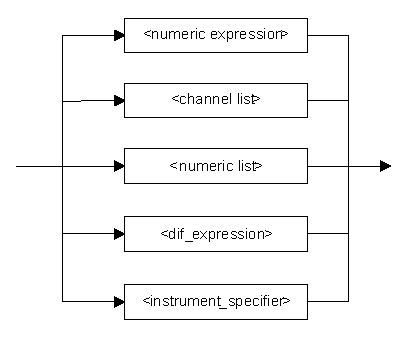
\includegraphics[scale=1]{Figuri/scpi_ro_3.eps}
 \caption{Sintaxa expresiilor}
 \label{fig5}
\end{figure}

\^{I}n cadrul expresiilor, "spa\c{t}iile albe" asa cum sunt denumite \^{i}n standardul IEEE 488.2, sunt permise \^{i}ntre orice elemente lexicale. Prin element lexical se \^{i}n\c{t}elege un operator, un semn de punctua\c{t}ie, cuv\^{a}nt cheie, tip de valoare.

\subsection{Expresii numerice}
O expresie numeric\u{a} este o colec\c{t}ie de termeni care evalueaz\u{a} un num\u{a}r, un vector sau un alt tip de informa\c{t}ie.

Sintaxa unei expresii numerice:
\begin{itemize}
	\item un operator numeric \textless numeric\_operator\textgreater;
	\item un operator numeric unar \textless unar\_numeric\_operator\textgreater;
	\item o variabil\u{a} \textless variable\textgreater sau \textless trace\_name\textgreater;
	\item o list\u{a} de canale \textless channel\_list\textgreater
\end{itemize}

\section{Raportarea st\u{a}rii}
Un dispozitiv SCPI trebuie s\u{a} includ\u{a} un registru de stare special - OPERation precum \c{s}i un registru de stare dat\u{a}/semnal QUEStionable \^{i}mpreun\u{a} cu condi\c{t}iile asociate, evenimente \c{s}i comenzi de activare.

De asemenea se stabilesc anumite cerin\c{t}e adi\c{t}ionale pentru instrumentele care suport\u{a} ori INSTrumente logice multiple ori modele de TRIGger cu posibilit\u{a}\c{t}i extinse. \^{I}n mod normal un registru de stare trebuie s\u{a} intre \^{i}ntr-o valoare \^{i}ntreag\u{a} de 16 bi\c{t}i cu bitul cel mai semnificativ totdeauna egal cu zero (logic pozitiv).
